%% Content from http://zhenti.kaoyan.eol.cn/
%% Format by PythonShell
%% 2014-01-08

\section{Writing}
\textbf{Part A}

\textbf{51. Directions:}

\qquad Write an e-mail of about 100 words to a foreign teacher in your college, inviting him/her to be a judge for the upcoming English speech contest.

\qquad You should include the details you think necessary.

\qquad You should write neatly on the ANSWER SHEET 2.

\qquad Do not sign your own name at the end of the e-mail. Use ``Li Ming'' instead.

\qquad Do not write the address. (10 points)

\vspace{6pt}

\textbf{Part B}

\textbf{52. Directions:}

\qquad Write an essay of 160-200 words based on the following drawing .In your essay, you should

\qquad 1) describe the drawing briefly.

\qquad 2) interpret its intended meaning ,and

\qquad 3) give your comments.

\qquad You should write neatly on the ANSWER SHEET 2. (20 points)

\begin{center}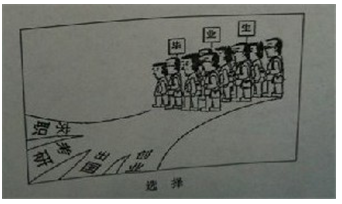
\includegraphics[width=14cm]{8.png}\end{center}